\chapter[MC event generation]{Monte-Carlo event simulation}
\label{chap:MC}

Although nowadays a very elegant and complete theoretical description of particle physics exists, it is not always evident how to translate this theory in actual predictions to compare with measurements. Moreover, on the case of hadronic colliders, as the LHC, it is even more difficult due to the characteristics of the strong interaction. On this subject, a set of tools and approaches have been developed in order to be able to make accurate predictions from theory that could be directly tested for experimentally, for example by ATLAS or CMS experiments. In the present chapter, such tools and formalisms and a set of studies comparing their predictions to data are described. 

\section{Monte-Carlo simulations}
\label{sec:MC}

The Monte-Carlo (MC) simulations use random numbers and large samplings to calculate mathematical quantities in complex configurations, as integrals or probabilities. The typical example is on how to calculate the integral of a one-dimensional function. Several random points can be thrown in the Cartesian plane and count how many of them are under the function. Then the integral of the function will be proportional to the fraction of points under the curve to the total used points. Larger the number of points, closer the estimation to the real value. An illustration of the procedure is shown in figure~\ref{fig:mc_int}.

\begin{figure}[!Hhtbp]
  \begin{center}
    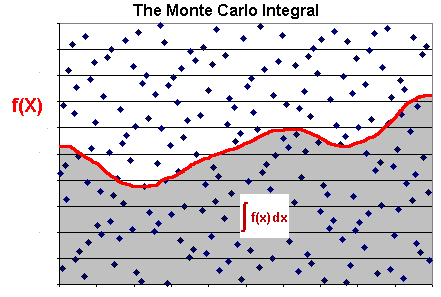
\includegraphics[width=0.6\textwidth]{figs/mc_integral.png}
    \caption{Integration using Monte-Carlo methods. The points in the plane have been chosen randomly. The integral of the plotted function is proportional to the ratio of points under the curve to the total number of used points.}
    \label{fig:mc_int}
  \end{center}
\end{figure}

A similar method is utilized to simulate proton-proton collisions. This simulation is used to generate ``random'' events and to calculate quantities, as the cross section, for a given physical process. Each event represents the final state of a collision, i.e. the set of particles produced from the collision and detected by the apparatus. Such simulations comprehend different steps: first, the partonic processes making reference to the interaction between the partons inside the proton; second, the hadronization of the particles produced from parton interactions; and third, the simulation of the interaction between the hadrons (from second step) and the detector materials. Such events are used to evaluate predictions from theory in the frame of a specific experiment. Whereas the hadronization and detector simulation are well-known physical processes, new theoretical predictions rely basically on the partonic level, where the fundamental interaction processes take part.

\subsection{Parton simulation}
\label{sec:parton}

The parton model was initially proposed by Richard Feynman in 1969~\cite{Feynman:1969ej}, as a method to understand collisions of non-fundamental particles. The model considers a composed particle, as a proton or a neutron, formed by a given number of point-like fundamental particles. When a collision occurs the point-like particles inside have a major probability to scatter. For example, when an electron collides with a proton, most of the interactions will be between the electron and the fundamental charged components of the proton, $u$ and $d$ quarks. This ``hard'' components are called valence quarks. Surrounding them, there is the sea of quarks and gluons.

However, as the energy of the collision increases the probability to scatter a sea component, quark or gluon, increases. In addition, even if the valence quarks of a proton are the $u$ and $d$ quarks, heavier quarks can appear in the sea, as the $b$, $c$ or $s$ quarks. The probability to interact with a component, a valence one or from the sea, is described by parton distribution function, commonly called PDF. A PDF function $f\equiv f(x,Q^{2})$ represents the number density of a given quark or gluon as a function of the resolution scale $Q^{2}$ and the fraction of momentum carried by the parton $x$. The determination of a PDF is done via a fit of large data samples from experiments specifically designed to test the inner structure of nucleons. The SLAC center (Stanford Linear Accelerator Center)~\cite{SLACTDR}, in California, United States, first probed the existence of partonic structure inside nucleons using leptons as probes scattered against nucleons, with experiences known as deep inelastic scattering (DIS) experiments~\cite{Whitlow:227258}. Another important experiment was the HERA~\cite{DESY-HERA-81-10} accelerator at DESY in Hamburg, Germany, which used electrons to study the inner structure of protons~\cite{Chekanov:2009na}.

In figure~\ref{fig:MSTW} the Martin-Stirling-Thorne-Watt~\cite{Martin:2009iq} (MSTW) PDF for two resolution scales is shown, taken from~\cite{Martin:2009iq}. The MSTW PDF is one of the experimental fits combining data from DIS and HERA. From this PDF, it is shown that $u$ and $d$ quarks carry the most of the momentum of the proton. The rest of the momentum is spread mainly over a huge amount of gluons and some, less probable, sea quarks as $\bar{u}, \bar{d}$ or $c$ and $s$. One important feature is that the composition of the proton changes depending on the resolution scale. At $Q^{2}= 10\, \text{GeV}^{2}$ there is no probability to find a $b$-quark in the proton while at $Q^{2}= 10^{4}\, \text{GeV}^{2}$ there is a non-negligible probability to find it.

\begin{figure}[!Hhtbp]
  \begin{center}
    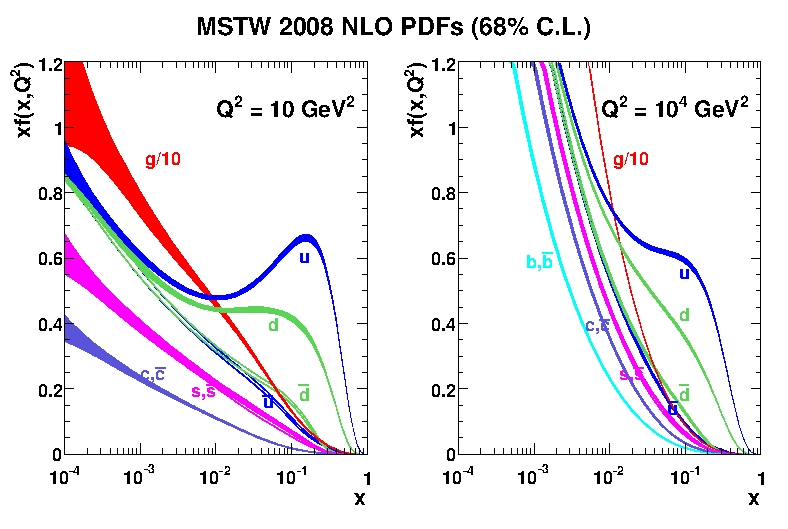
\includegraphics[width=0.9\textwidth]{figs/mstw2008nlo68cl_allpdfs.jpg}
    \caption{Martin-Stirling-Thorne-Watt proton PDF for $Q^{2}= 10\, \text{GeV}^{2}$ [left] and $Q^{2}= 10^{4}\, \text{GeV}^{2}$ [right]. $x$ is the fraction of momentum carried by the parton and $f(x,Q^{2})$ the PDF function~\cite{Martin:2009iq}.}
    \label{fig:MSTW}
  \end{center}
\end{figure}

Two other important PDF fits are CTEQ~\cite{Nadolsky:2008zw} and NNPDF~\cite{Ball:2010de}. Together with MSTW, they are the most used PDF sets in the CMS experiment for MC production. 

The knowledge of the proton content allows to compute the cross section of processes proton-proton collisions. This cross section depends of the momentum carried by each parton inside the parton, and are modulated by the probability of the interaction between different quarks during the collision.

For a scattering process, the hard part of the differential cross section can be written as,

\begin{eqnarray}
  \label{eq:DiffXS}
  d\sigma_{ij\rightarrow lm} & = & \left( \int_{0}^{1}\int_{0}^{1}f_{i}(x_{i},Q^{2})f_{j}(x_{j},Q^{2})dx_{i}dx_{j} \right) \nonumber \\  
 & \times & \frac{d^{3}p_{l}}{(2\pi)^{2}2E_{l}}\frac{d^{3}p_{m}}{(2\pi)^{2}2E_{m}}\delta^{4}\left( p_{i}+p_{j}-p_{l}-p_{m} \right) \nonumber \\  
 & \times & |\mathcal{M}_{ij\rightarrow lm}|^{2}
\end{eqnarray} where $f_{i,j}$ corresponds to the PDF's of the initial partons. $\mathcal{M}_{ij\rightarrow lm}$ is the matrix element of the process which is the part of the S-matrix that contains the amplitude of the process, and governs the transition from the initial to the final state~\cite{opac-b1131978}. The matrix element could account effectively for all processes mediating the transition from the initial to a given final state, but in practice it is calculated only with a given number of processes. The calculation can achieve different levels, usually tree level or Leading Order (LO), but modern calculation could arrive, depending on the process, to one loop or Next-to-Leading-Order (NLO) or even two loops the  Next-to-Next-to-Leading-Order (NNLO). This limit depends exclusively on the feasibility of the theoretical calculations. Figure~\ref{fig:LOpNLO} shows an example of a leading order and its corresponding NLO diagrams for a fermion scattering.

\begin{figure}[!Hhtbp]
  \begin{center}
    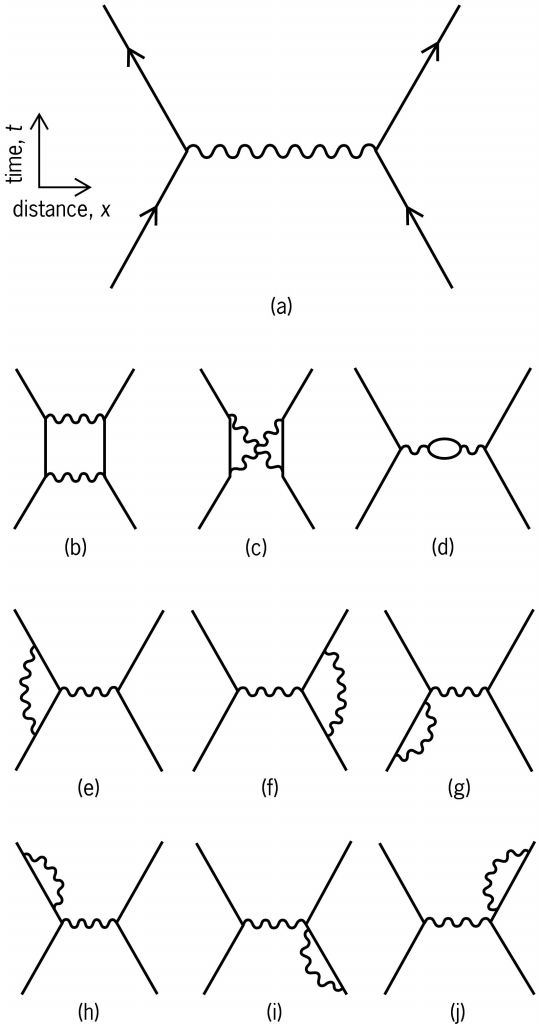
\includegraphics[width=0.7\textwidth]{figs/Feynman_diagrams.jpg}
    \caption{LO (a) and NLO (b)-(j) processes contributing to fermions scattering. Several processes have to be considered in order to have accurate predictions for experimental measurements.}
    \label{fig:LOpNLO}
  \end{center}
\end{figure}

Parton simulations try to simulate the interactions between partons in hadronic collisions. They are the basic level for many particle physics simulation of events, where the basic pieces, as the matrix element of the quarks interaction, are calculated.

\subsection{Hadron simulation}
\label{sec:hadron}

Quarks produced in a collision are not seen freely due to the strong interaction. They will take quarks from vacuum to form hadrons. What reaches the detector as final state are the stable hadrons resulting from the hadronization process. From a single parton several hadrons can result, producing a shower of particles, as seen in figure~\ref{fig:Hadr}. Two main processes are simulated, the showering that corresponds to radiations emitted by quarks, from initial or final state, and hadronization the process of forming hadrons from quarks and gluons. 

As QCD strong interaction imposes several theoretical restrictions to have a first principle understanding of these phenomena, the description of hadronization relies on the construction of effective models. There are basically two main models to simulate hadronization and showering of quarks and gluons, both giving comparable predictions. It is important to remark that this is a crucial step in simulations as from an accurate hadron production simulation depends the correctness of MC description of jets.

\begin{figure}[!Hhtbp]
  \begin{center}
    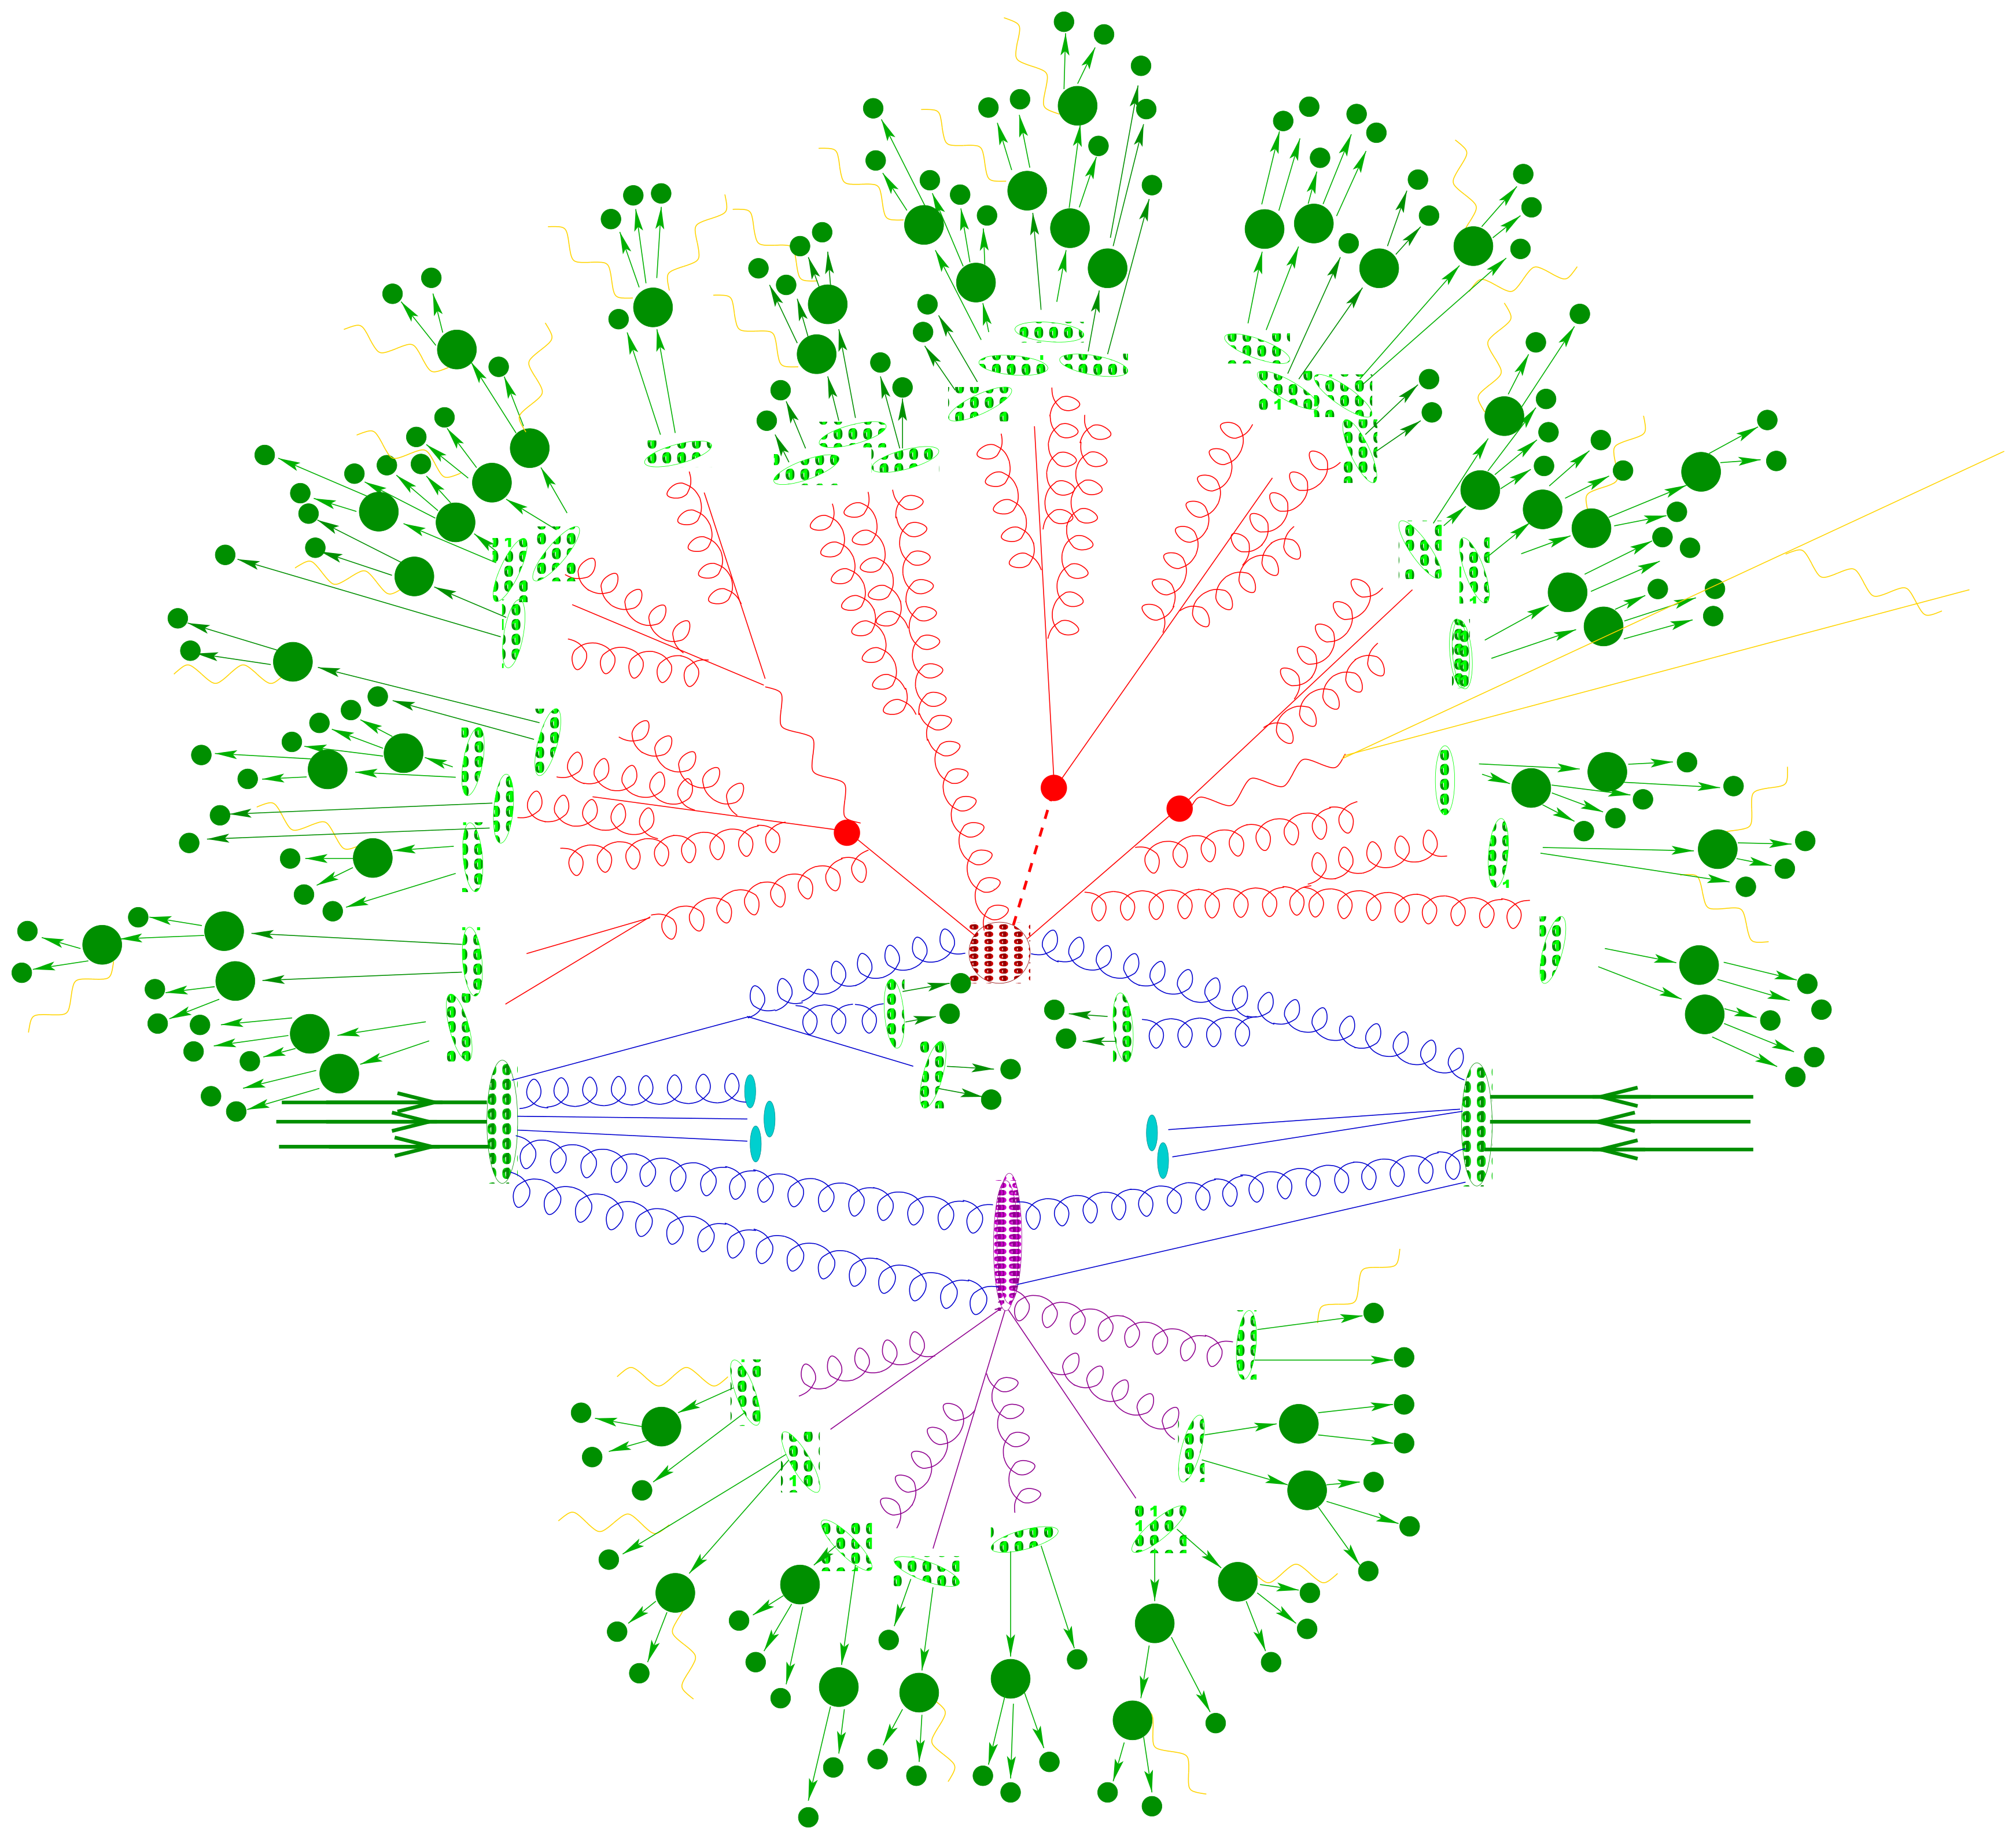
\includegraphics[width=\textwidth]{figs/parton_shower.png}
    \caption{Graphical representation of the hadronization process of partons resulting from a proton-proton collision. The biggest green ellipses, preceded by three green arrows, represent the initial protons. The small green circles inside them represent the partons inside the protons. The big red circle, with small red circles inside, represent the hard interaction from partons (in blue lines). The hard interaction produces three particles, red full small circles, that decay afterward. The red lines represent the decay products from the particles produced in the hard interaction, and the additional particles produced from showering. Final hadrons are drawn in the most exterior part of the graph. These final hadrons are represented by the small full green circles.}
    \label{fig:Hadr}
  \end{center}
\end{figure}
%\begin{TOINCLUDE}Figure to illustrate to hadronization process\end{TOINCLUDE}

\subsection{Detector simulation}
\label{sec:detector}

After final particles from a collision are simulated, the next step is to simulate the interaction of these particles with the detector. The principle is that the detector response should be simulated as close as possible to the real detector. In that sense, the objective is to have a detector response using MC simulations as with real data. However, not everything can be simulated. For example, during data taking different problems might arise (subdetector misbehaving, dead cells, etc.) that can not be adjusted in MC simulation, and needs further correction and tuning. Moreover, in practice, MC simulations for ATLAS and CMS experiments are prepared before data taking. Then, if one wants to reproduce precisely the details of what happened with the detector during the data taking, MC simulation should be redone to reproduce the data taking particularities. 

CMS has used GEANT 4~\cite{Agostinelli:2002hh} software to simulate the detector. Precise implementation of detector geometry was done in order to correctly simulate each subdetector, their details as size, number of channels, cells, electronic cards, were taken into account. This simulation allows to get, as for data, the same output from the detector to be used for the reconstruction and identification of the objects. 

%MC simulations are always being corrected to match correctly the real experimental conditions. Moreover for complicated objects as jets, with many subdectectors information combined, or jet b-tagging that depends strongly of finding second vertices, it is easier to find in \textit{optimal} MC simulation conditions than in experimental reality.

\section{Tools}
\label{sec:tools}

There are several tools on the market to perform the different steps of MC simulations of proton-proton collisions. I'll briefly describe some of them, the most used in CMS.

\subsection{Matrix-element generators}
\label{sec:ME}

Regarding parton simulation, MadGraph~\cite{Alwall:2014hca, Alwall:2011uj} package is one of the most widely used both by experimental and theoretical particle physics communities. It calculates matrix-elements, LO cross sections and particle widths. With such information, it generates MC events for parton collisions. 

The latest series of releases also include an additional package to perform NLO QCD corrections to SM processes. The framework also includes the possibility to work with BSM models, making it a powerful tool for evaluating predictions from them. Another parton generator is POWHEG, in its most recent version POWHEG BOX~\cite{Nason:2004rx, Frixione:2007vw, Alioli:2010xd}, that is specially accurate to simulate events with top quarks. %It is well known that this generator gives a better agreement between data and MC in top physics.

In CMS, all physics groups analyzing data collected by the experiment, have to do simulations of signals and backgrounds. For this purpose, MC simulation tools as MadGraph, need to be interfaced with the central CMS software CMSSW (CMS SoftWare). The generators group do this work preparing sets of validated code to be used later by CMS users. This group is also in charge of central MC production, the technical process of MC production of samples doing all the needed steps to obtain validated samples to compare with CMS data: parton generation, hadronization and detector simulation. 

Central production of samples using MadGraph is done via the generation of stand-alone packs of code used to launch parallelized production. This utility is known as gridpack. Gridpack generation must include all possible configurations needed for the CMS central production: settings to run within CMSSW in batch systems and additional physics requirements depending on the process to be generated. A special script has been put in place to allow users to do their own gridpack generation with small effort in terms of automatization of common tasks.

In addition, the generator group also provide constant support for users to test the validity of their production, their MadGraph configuration, the usage of the interface software in CMSSW and to test implementations of BSM models.

\subsubsection{Preparation of MadGraph production}

Any production of partonic MC samples with MadGraph relies on 4 key elements, a model and three production cards. In order to launch any event generation in MadGraph, a set of three cards has to be prepared. These cards are text files where the user can specify several parameters used by MadGraph to generate a sample. In more detail, the 4 elements are:
\begin{itemize}
\item Model: The implementation of the theoretical model according to which the production will be done. The implementation of a particle physics model, for computational calculations, is not a trivial task. Tools are available to perform this. MadGraph has incorporated as default the model implementation developed by FeynRules~\cite{Alloul:2013bka}, the Universal FeynRules Output (UFO)~\cite{Degrande:2011ua}. A complete set of tools to facilitate the implementation of theoretical models for computational work with different packages was developed in FeynRules. MadGraph includes by default the implementation of the SM and the Minimal SuperSymmetric Model (MSSM), but in order to generate events for private models, its implementation has to be provided. The facility to generate events for any model has been one of the most appealing features of MadGraph for the particle physics community.
\item Process card: In this card, the user defines the model to be used and the process to be generated. In general, the process definition could use the definition of multi-particle labels that MadGraph utilizes to loop over all the particles contained in the label. Multi-particle labels are variables defined by the user to design sets of particles from the model. Figure~\ref{fig:ProcCard} shows the lines contained in the process card to generate $t\bar{t}$ with 0 and 1 additional jet. In this example, the proton is defined as a multi-particle label containing all the quarks (except the top) and the gluon. Afterward, positively and negatively charged leptons are grouped under multi-particle labels ``l+'' and ``l-''. Similar labels are declared for neutrinos and anti-neutrinos. After the declaration of labels, the process for the production is declared, in this case \ttbar~production with 0 and 1 additional jet.
  \begin{figure}[!Hhtbp]
    \begin{center}
      \begin{minipage}[c]{0.45\textwidth}
\begin{verbatim}
import model sm
# Define multiparticle labels
define p = u c s d b u~ c~ s~ d~ b~ g
define j = p
define l+ = e+ mu+ ta+
define l- = e- mu- ta-
define vl = ve vm vt
define vl~ = ve~ vm~ vt~
# Specify process(es) to run
generate p p > t t~  @0
add process p p > t t~ j @1
# Output processes to MadEvent directory
output -f
\end{verbatim}
        \end{minipage}
          \caption{MadGraph process card example.}
          \label{fig:ProcCard}
      \end{center}
    \end{figure}
    
  \item Parameters card: This card is used to set the parameters of the model invoked for the production. Following the example of top pair production, it might be interesting to produce different samples varying the top mass. In figure~\ref{fig:ParamCard} an extract of the card that controls the masses of the particles in the model is shown. The first column refers to the PDG ID of the particles, 6 for the top quark, and the second column is the value of the mass. In this case, the top mass has been set to 172.5 \GeVcc.
    \begin{figure}[!Hhtbp]
      \begin{center}
        \begin{minipage}[c]{0.45\textwidth}
\begin{verbatim}
###################################
## INFORMATION FOR MASS
###################################
Block MASS 
    4 1.420000e+00 # MC 
    5 4.800000e+00 # MB 
    6 1.725000e+02 # MT 
   11 5.110000e-04 # Me 
   13 1.056600e-01 # MM 
   15 1.777000e+00 # MTA 
   23 9.118800e+01 # MZ 
   25 1.250000e+02 # MH 
\end{verbatim}
        \end{minipage}
          \caption{Extract of MadGraph parameters card. The first column refers to the PDG ID of the particles, 6 for the top quark, and the second column is the value of the mass. In this case, the top mass has been set to 172.5 \GeVcc.}
          \label{fig:ParamCard}
      \end{center}
    \end{figure}

  \item Run card: In the run card several settings can be fixed related to the generation of the events. For example, the center of mass energy or the minimal and maximal $\Delta R$ between jets. For generation of events requiring more than one additional extra jet, a parameter called xqcut can also be set in this card. This parameter is relevant for the merging procedure, important to avoid double counting, a topic that will be discussed in section~\ref{sec:Merging}. In figure~\ref{fig:RunCard} an extract of a run card is shown, where the parameters corresponding to the center of mass energy of the collision, the number of events to be generated, the gridpack generation, the choice of PDF set and the merging procedure are displayed.
    \begin{figure}[!Hhtbp]
      \begin{center}
        \begin{minipage}[c]{0.7\textwidth}
\scriptsize
\begin{verbatim}
#*********************************************************************
# Run to generate the grid pack                                      *
#*********************************************************************
  .true.     = gridpack  !True = setting up the grid pack
#*********************************************************************
# Number of events and rnd seed                                      *
#*********************************************************************
  1000       = nevents ! Number of unweighted events requested 
      0       = iseed   ! rnd seed (0=assigned automatically=default))
#*********************************************************************
# Collider type and energy                                           *
#*********************************************************************
        1     = lpp1  ! beam 1 type (0=NO PDF)
        1     = lpp2  ! beam 2 type (0=NO PDF)
     6500     = ebeam1  ! beam 1 energy in GeV
     6500     = ebeam2  ! beam 2 energy in GeV
#*********************************************************************
# PDF CHOICE: this automatically fixes also alpha_s and its evol.    *
#*********************************************************************
 'cteq6l1'    = pdlabel     ! PDF set  
#*********************************************************************
# Matching - Warning! ickkw > 0 is still beta</div>
#*********************************************************************
 1        = ickkw            ! 0 no matching, 1 MLM, 2 CKKW matching
 1        = highestmult      ! for ickkw=2, highest mult group
 1        = ktscheme         ! for ickkw=1, 1 Durham kT, 2 Pythia pTE
 1        = alpsfact         ! scale factor for QCD emission vx
 F        = chcluster        ! cluster only according to channel diag
 F        = pdfwgt           ! for ickkw=1, perform pdf reweighting
#*********************************************************************
# Jet measure cuts                                                   *
#*********************************************************************
 20   = xqcut   ! minimum kt jet measure between partons
#*********************************************************************
\end{verbatim}
\normalsize
        \end{minipage}
          \caption{Extract of MadGraph run card.}
          \label{fig:RunCard}
      \end{center}
    \end{figure}

\end{itemize}


\subsubsection{MadGraph release validation}

MadGraph is a very dynamic tool, where the input from the users is being taken into account permanently: users give reports of possible bugs or recommendations in the way tool works. New releases of MadGraph are constantly delivered to solve found issues or to improve weaknesses. For CMS production, not every new release is automatically incorporated. In order to begin using a new release a validation procedure is done, which is time and resources demanding. Basic processes of the SM are considered using the last release used by CMS and then compared to the new release. Such comparison is performed to control that predictions from both releases are identical, for processes where no changes have been performed between both releases. 

For example, one of the control processes for this validation is the SM production of a \Z~boson that decays into neutrinos produced with extra jets. MadGraph is able to produce extra jets up to a multiplicity of 4. In figure~\ref{fig:ZRelVal1} the comparison between samples produced with MadGraph 1.4.8 and 1.5.11 is displayed. The results of both releases are equivalent for the specific considered process.

\begin{figure}[!Hhtbp]
  \begin{center}
    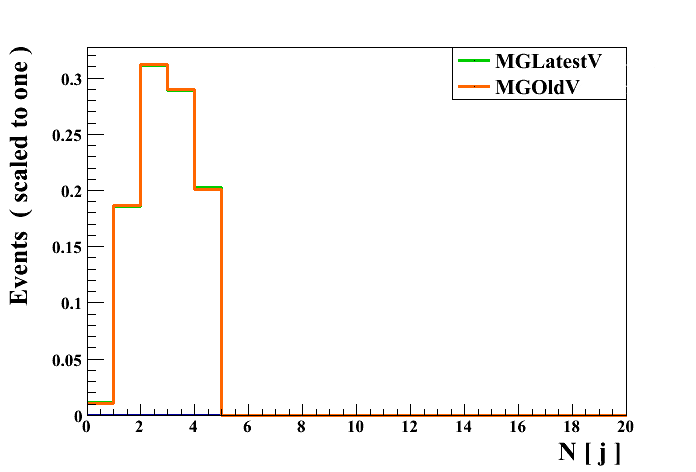
\includegraphics[width=0.45\textwidth]{figs/ZjetsRelVal0.png}
    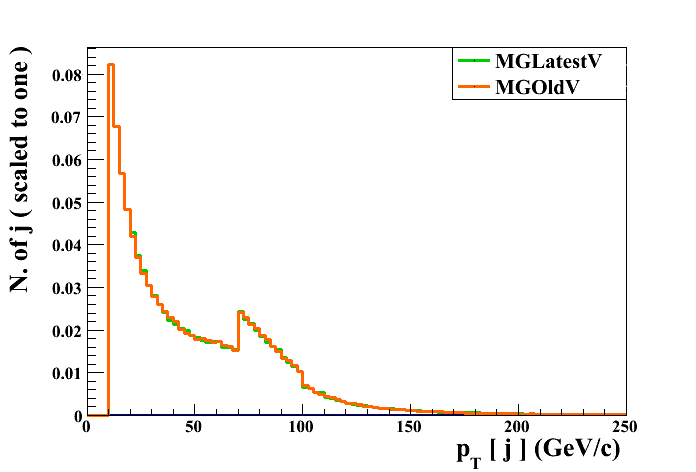
\includegraphics[width=0.45\textwidth]{figs/ZjetsRelVal1.png}
    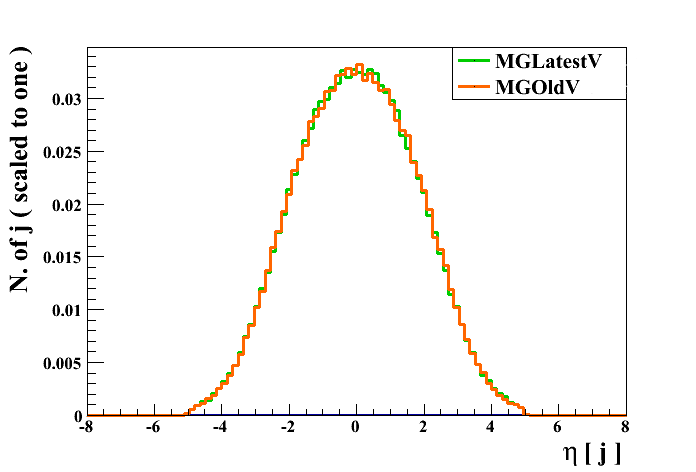
\includegraphics[width=0.45\textwidth]{figs/ZjetsRelVal2.png}
    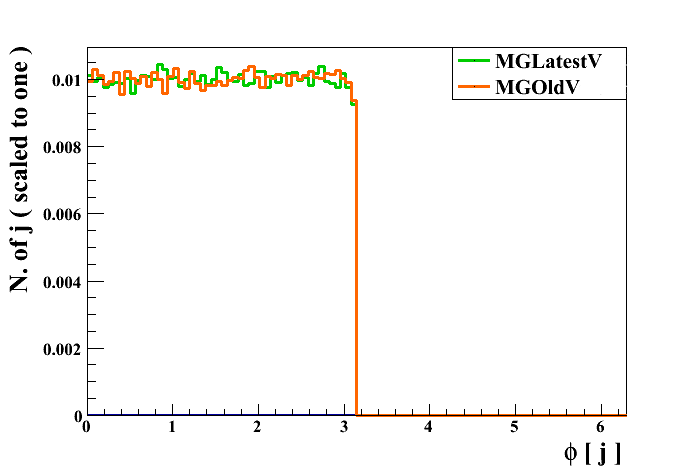
\includegraphics[width=0.45\textwidth]{figs/ZjetsRelVal3.png}
    \caption{Comparison between 1.4.8 (MGOldV) and 1.5.11 (MGLatestV) MadGraph releases for SM \Z+jets production with \Z~decaying into neutrinos. Number of jets [left-up], $p_{T}$ of jets [right-up], $\eta$ of jets [left-down] and $\phi$ of jets [right-down]. As expected, no deviation is observed.}
    \label{fig:ZRelVal1}
  \end{center}
\end{figure}

In addition, figure~\ref{fig:ZRelVal2} shows two global variables, the missing energy and the total hadronic transverse energy (defined in equation~\ref{eq:METHT}), for the same process where the validation was performed.

\begin{equation}
  \label{eq:METHT}
  \slashed{E}_{T}=|\sum_{visible\; particles}\vec{p}_{T}|, \; \; H_{T}=\sum_{hadronic\; particles}|\vec{p}_{T}|
\end{equation}

\begin{figure}[!Hhtbp]
  \begin{center}
    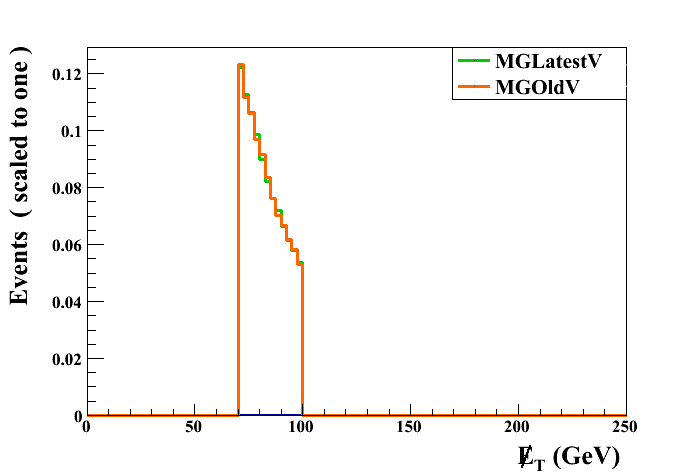
\includegraphics[width=0.45\textwidth]{figs/ZjetsRelVal8.png}
    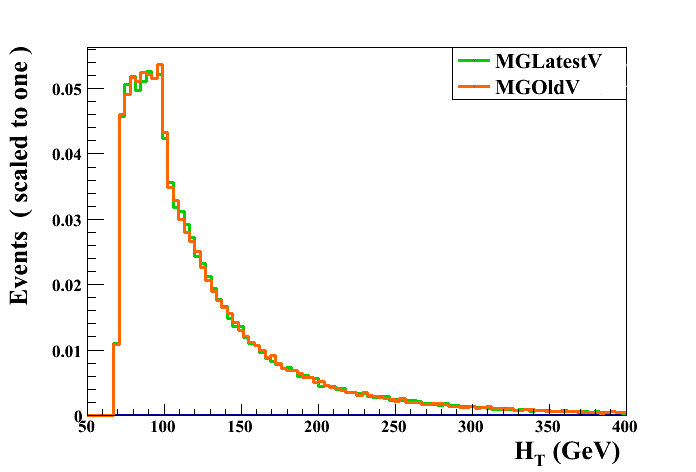
\includegraphics[width=0.45\textwidth]{figs/ZjetsRelVal9.png}
    \caption{Comparison between 1.4.8 (MGOldV) and 1.5.11 (MGLatestV) MadGraph releases for SM \Z+jets production with \Z~decaying into neutrinos. Missing energy [left] and total hadronic transverse energy [right]. No difference is seen between both versions.}
    \label{fig:ZRelVal2}
  \end{center}
\end{figure}

In the study shown in the mentioned figures, there is no difference between the two compared releases for the processes used.

\subsubsection{Incorporating new releases improvements}

New MadGraph releases are interesting not only because of bugs being fixed but also because they include new features and improvements. For example, latest set of releases include NLO corrections for SM processes, improvement not present before. NLO corrections are crucial to do precise measurements, that is one of the major interests in various SM sectors. Top physics has become a very important sector to perform precise measurements. Any small deviation of SM predictions related to the top quark could be related to the presence of BSM physics. To this extent, there is a growing need to have better MC simulations of top quark processes.

From a technical point of view, a complete simulation of top decay chain was not feasible at MadGraph level. It was extremely time and CPU consuming for old MadGraph releases. Modern releases (from MadGraph 5) have improved the performance of these calculations but also have included new tools that allow to simulate the entire top decay at parton level chain with high precision and small resources. One of these tools is MadSpin~\cite{Artoisenet:2012st, Frixione:2007zp}, which was developed to preserve spin correlations between decay products. However MadGraph alone is able to simulate the top decay, it is still extremely CPU and time consuming, and then, not suitable for big central production at CMS. On the other hand, decaying the top quark with Pythia erases all spin correlations. In CMS, MadSpin has been included in the gridpack generation production mainly to generate top pair production samples. MadSpin is the modern version of the old DECAY tool, that did not preserve spin correlations.

However to consider using MadSpin in CMS, an improvement with respect to former samples should be shown. MadSpin is expected to have the same results as MadGraph, but with an improvement in terms of computational resources consumption. Figure~\ref{fig:MS1} shows the top quark mass reconstructed from its hadronic decay ($b$, $u$ and $\bar{d}$ quarks). This figure demonstrate that MadSpin and MadGraph produce comparable results with a non-zero top width, while DECAY gives a zero width. The $\Delta R$ between the positively and negatively charged decay products of the \W~bosons produced in top pair events is displayed in figure~\ref{fig:MS2}. This observable is different in the case where there are or no spin correlations. 

\begin{figure}[!Hhtbp]
  \begin{center}
    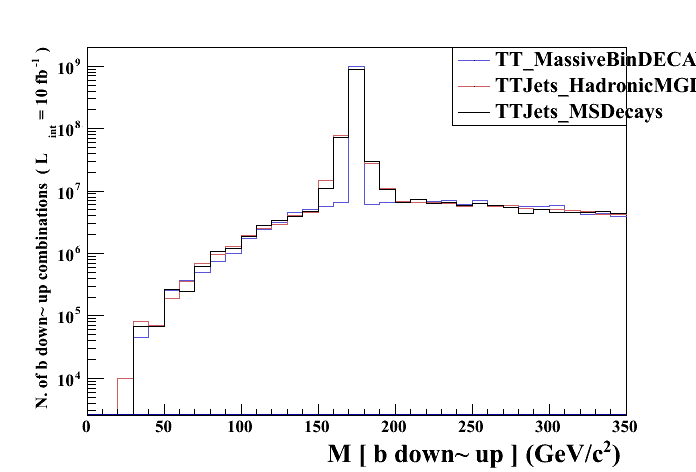
\includegraphics[width=0.65\textwidth]{figs/TT_MadSPin_1.png}
    \caption{Top mass reconstructed from its hadronic decay using different tools to simulate the top decay for $t\bar{t}$ events at $\sqrt{s}=8$ TeV. MadSpin and MadGraph correctly reproduce the top width.}
    \label{fig:MS1}
  \end{center}
\end{figure}

\begin{figure}[!Hhtbp]
  \begin{center}
    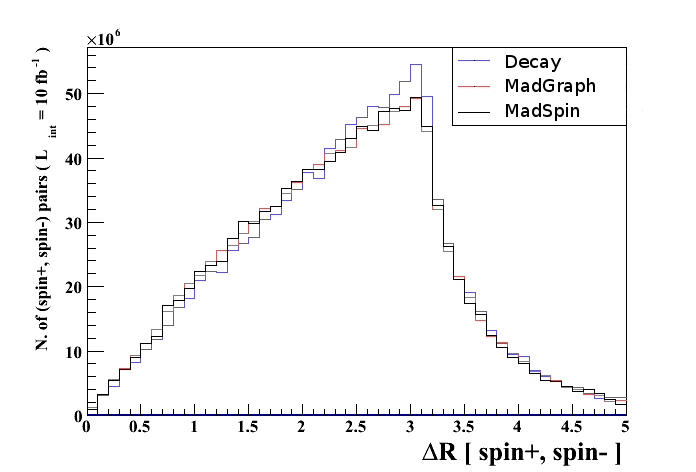
\includegraphics[width=0.65\textwidth]{figs/TT_MadSPin_2.png}
    \caption{$\Delta R$ from positively and negatively charged decay products using different tools to simulate the top decay for $t\bar{t}$ events at $\sqrt{s}=8$ TeV. MadSpin and MadGraph produce different results than the DECAY tool, as these first two preserve spin correlations.}
    \label{fig:MS2}
  \end{center}
\end{figure}

\subsection{Hadron generators}
\label{sec:Had}

Taking as input partonic events, hadron generators perform their corresponding showering and hadronization. The most used hadronizers in CMS are Pythia~\cite{Sjostrand:2006za}, in releases 6 and 8, and Herwig ++~\cite{Bahr:2008pv}. They are used to simulate a wide range of SM processes simulation. They can be used as MC generators, without the parton step, which is specially used to simulate QCD processes.

Hadronization processes are QCD mediated. As the strong force is a non-perturbative interaction, different hadrons simulations implement different effective models. Reason why when comparing simulations to data, different hadron generators are used in order to understand the set of data independently from the hadronization model. 

\subsubsection{Interface between partonic and hadronic generation of events}
\label{sec:Merging}

Matrix element (ME) generation is responsible for the simulation of the hard processes. This corresponds to generating all the final quarks and gluons coming from the collision. Parton showering (PS) is responsible for the simulation of ``soft'' processes coming from the strong interaction. For example, an initial or final quark can radiate a gluon that will lead to additional jets in the event. The generation of extra jets (coming from extra quarks or gluons) can suffer from an overlap between the ME and PS. In figure~\ref{fig:PSME}, a graphical description of the procedure followed by ME and PS to add extra jets to a process is shown. 

\begin{figure}[!Hhtbp]
  \begin{center}
    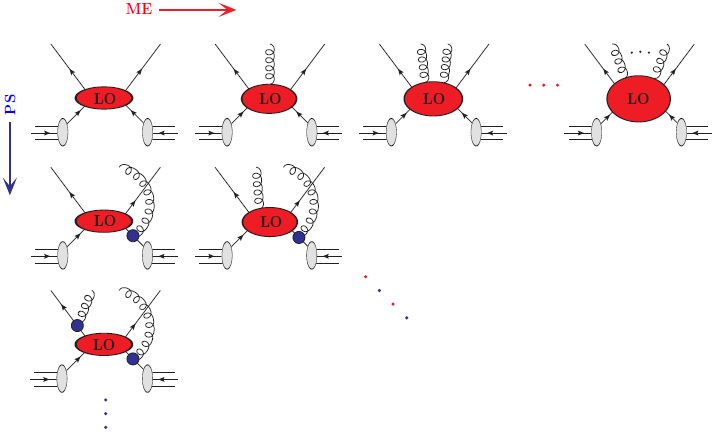
\includegraphics[width=0.75\textwidth]{figs/PSMEInterface.png}
    \caption{ME and PS contributions to events with several partons in the final state in a leading order MC simulation.}
    \label{fig:PSME}
  \end{center}
\end{figure}

This overlap can lead to double counting events, which has as consequence an overestimation of the cross section of the process. To solve this issue a procedure has been designed to study the overlap between MadGraph and Pythia. This procedure is known as merging~\cite{Alwall:2007fs, Alwall:2008qv, Lavesson:2007uu}. It is based on the application of one or two cuts to separate hard and soft phase space, hard region being generated by ME and soft region by PS. MadGraph uses MLM merging formalism to do this task~\cite{Mangano:2001xp, Mangano:2006rw}. 

In general, the merging procedure follows a set of common steps:
\begin{itemize}
\item A jet algorithm is chosen and all relevant cross sections are calculated accordingly to the process under consideration. The calculation is performed for each final jet multiplicity. For example, when generating top pair production up to 4 additional jets, the cross section is calculated for $t\bar{t}$ with 0, 1, 2, 3, and 4 jets separately. 
\item ME samples are produced with a probability corresponding to their cross section.
\item Events or partons are rejected based on specific procedure requirement. For MLM formalism, events are rejected if not all partons are matched to jets. %MLM procedure will be described in details.
\item Parton shower is invoked, constrained to not produce any extra jet.0
\end{itemize}

MadGraph utilizes a MLM merging procedure with the $k_{T}$ jet algorithm. The MLM prescription proceeds as follows:
\begin{enumerate}
\item Generation of parton level events constrained to the requirements defined by the user:
  \begin{equation*}
    p_{T}^{parton}>p_{T}^{min}, \; |\eta^{parton}|<\eta^{max}, \; \Delta R_{partons}>R_{min}
  \end{equation*} where \textit{min} and \textit{max} stand for the minimal and maximal values required by the user for each variable.
\item The $k_{T}$ jet algorithm is used to find the jets of the event from partonic events. This first reconstruction uses a cut on the minimal $k_{T}$ distance as defined in equation~\ref{eq:kt}. This first minimal cut is set, by the user, in MadGraph with the variable xqcut (see~\ref{fig:RunCard}). $Q^{X}_{cut}$ will be used to refer to it. This cut is applied at generator level, what means that MadGraph will only deliver events where every pair of partons satisfy this requirement.
\item Running of the parton shower and hadronization over the partonic events, and rerunning of the jet algorithm with a different minimal $k_{T}$ distance. The second minimum, the $Q_{cut}$, is set in Pythia and is known as the merging scale. The two minima are chosen to be $Q_{cut}>Q^{X}_{cut}$. $Q_{cut}$ is also a generator cut at Pythia level. Pythia will give then only the events where every pair of hadrons pass this criterion.
\item Comparison of the set of jets obtained from step 2 and 3. If a jet from the parton event falls in a radius smaller than $1.5 \times R$ of a jet from the showered event, it is said to be matched to it ($R$ being the radius parameter of the jet algorithm). If a match is found for all partons the event is kept, otherwise is rejected.
\item Finally, if an event after hadronization has more jets than the generated partons, is discarded. %All events with more jets, after showering, than partons are finally discarded.   
\end{enumerate}

The goodness of the procedure depends of the choice of $Q_{cut}$ and $Q^{X}_{cut}$. The optimal values are highly dependent of several parameters, for example the $p_{T}$ of the partons or the center of mass energy of the collision. 

In general, for each process there are an optimal $Q_{cut}$ and $Q^{X}_{cut}$. But in principle there is no way to deduce them without producing the samples and performing the merging procedure. If the procedure was successful, it can be known only from the simulation results. Reason why, multiple generation of samples scanning both $Q_{cut}$ and $Q^{X}_{cut}$, are needed to find an optimal solution. As the main interest is to cover correctly the entire phase space with ME+PS, $Q^{X}_{cut}$ can be fixed and then $Q_{cut}$ scanned over it, with $Q_{cut}>Q^{X}_{cut}$. If no $Q_{cut}$ value optimize the merging procedure then another $Q^{X}_{cut}$ is used. 

The effectiveness of the merging procedure is checked through the differential jet rate (DJR) diagrams. Changing the merging scale $Q_{cut}$ might change the jet multiplicity of an event during the parton showering and hadronization by Pythia. In the DJR diagrams the transition between $n$ and $n-1$ jet multiplicities is examined as a function of the merging scale for different values of $n$. The $Q_{cut}$ controls the number of jets found in an event from parton showering. Its optimal value leads to a continuum in the transition phase between ME and PS. The choice of the correct merging scale is reflected in the smoothness of the transition between  $n$ and $n-1$ jet multiplicities. A non-optimal value leads to an under or overpopulation of the phase space. In both cases the sample does not represent a meaningful physics sample.

The optimal value of the merging scale, $Q_{cut}$, depends on several details of the generated events. For example, the minimal \pt~cuts set in the generation. But it strongly depends of the process and the center of mass energy of the collisions.

For MC samples generation for the run 2 of the LHC, optimal values for $Q_{cut}$ and $Q^{X}_{cut}$ should be found according to the increase of the center of mass energy from 8~TeV to 13~TeV. Figure~\ref{fig:TTJetsMerging} shows the DJR diagrams for $t\bar{t}$ production with up to 3 additional jets with MadGraph and Pythia 8. For this study $Q^{X}_{cut}=20$~GeV and the optimal $Q_{cut}$ was found to be 100 GeV (top figure). The result using $Q_{cut}=60$ GeV is also shown (bottom figure) where a discontinuity in the transition point between different jet multiplicities. In the figure at the bottom, the transition from 3 to 2 jets ($DJR(3\to 2)$) shows a discontinuity in the meeting point of blue-dashed and green-dashed curves, respectively 3 and 2 partons curves. In figure~\ref{fig:DYMerging} the same study is shown for Drell-Yan process with up to 3 additional jets at 13 TeV with MadGraph and Pythia 6. 

\begin{figure}[!Hhtbp]
  \begin{center}
    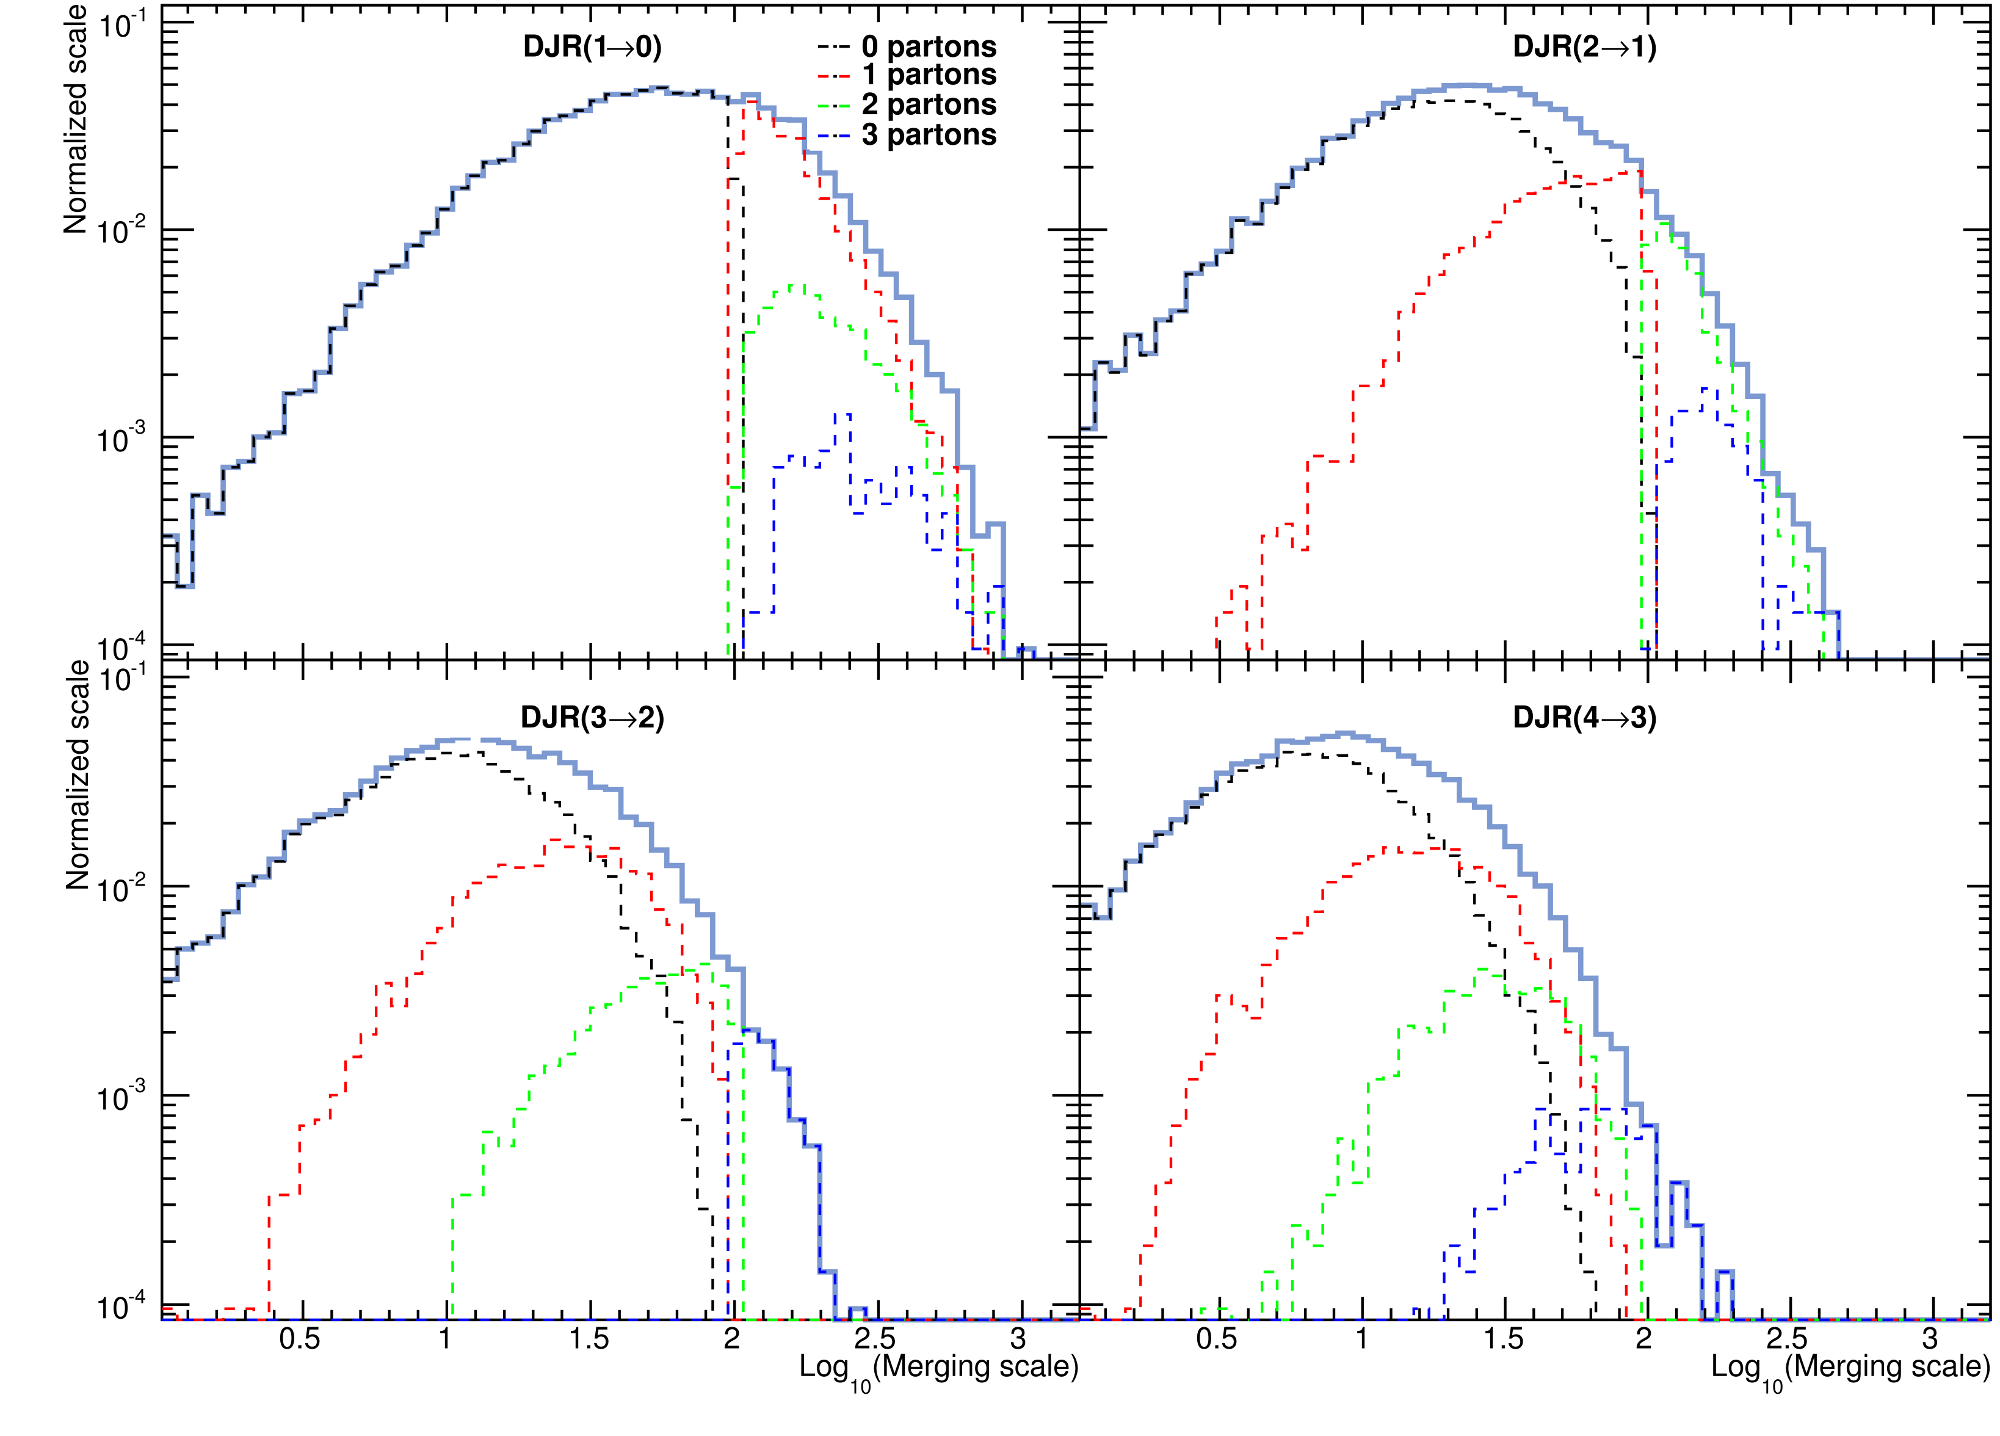
\includegraphics[width=0.85\textwidth]{figs/DJR_q100_xq20_TTJets13TeV.png}
    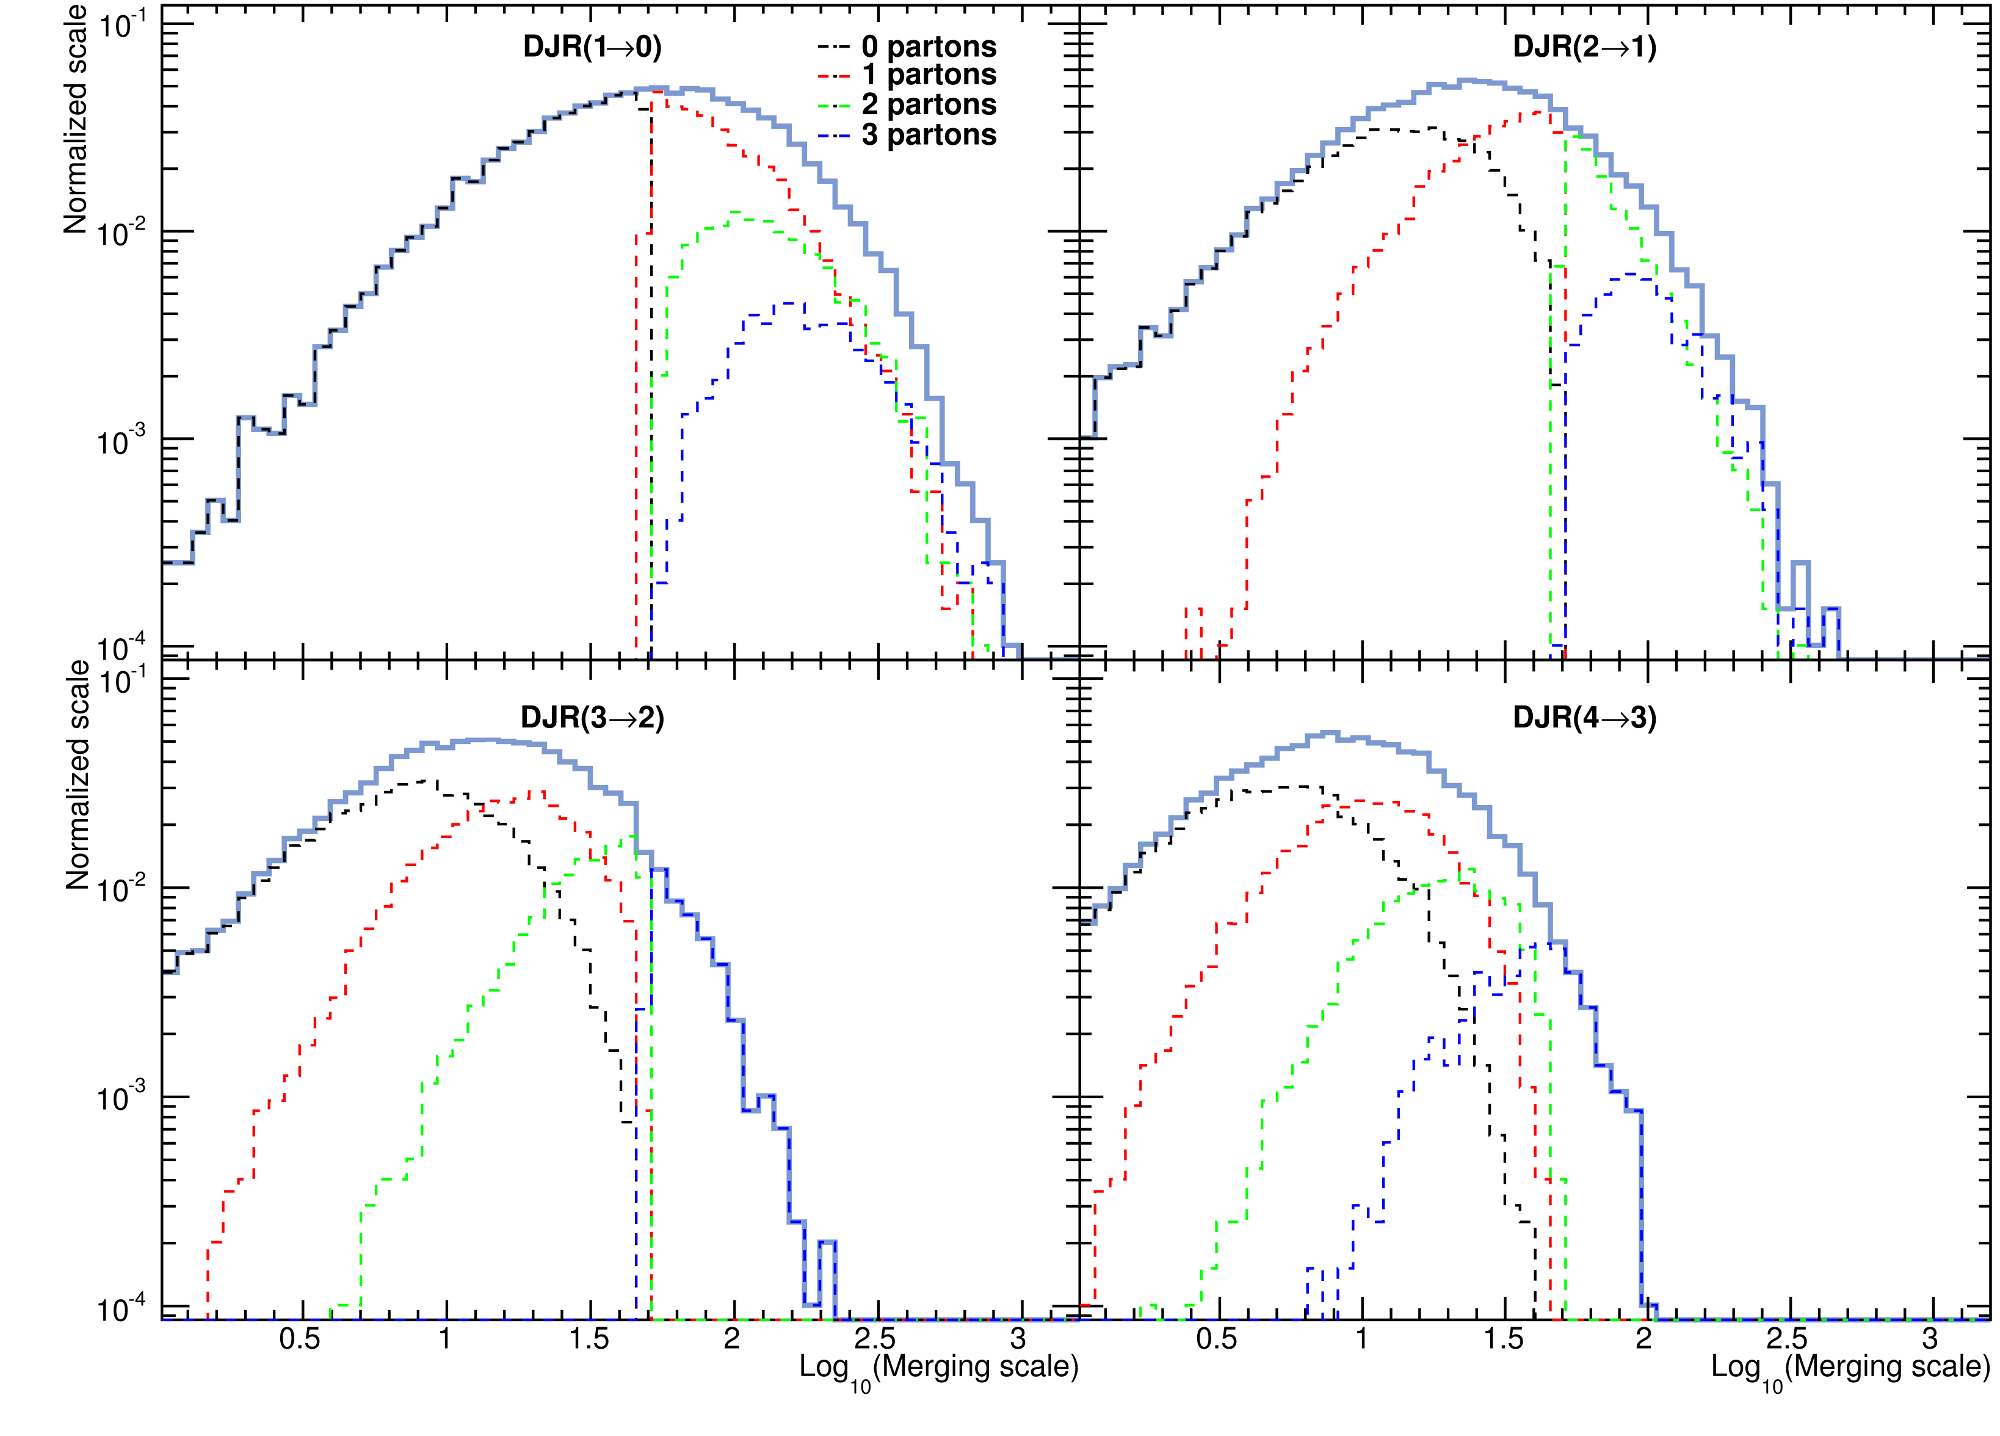
\includegraphics[width=0.85\textwidth]{figs/DJR_q50_xq20_TTJets13TeV.png}
    \caption{DJR diagrams for 13 TeV top pair production with $Q_{cut}=100$ GeV and $Q^{X}_{cut}=20$ GeV [optimal case] (top) and $Q_{cut}=60$ GeV and $Q^{X}_{cut}=20$ [non-optimal] (bottom). Bottom figure shows a discontinuity in the transition from 3 to 2 partons at the point where blue-dashed and green-dashed curves meet.}
    \label{fig:TTJetsMerging}
  \end{center}
\end{figure}

\begin{figure}[!Hhtbp]
  \begin{center}
    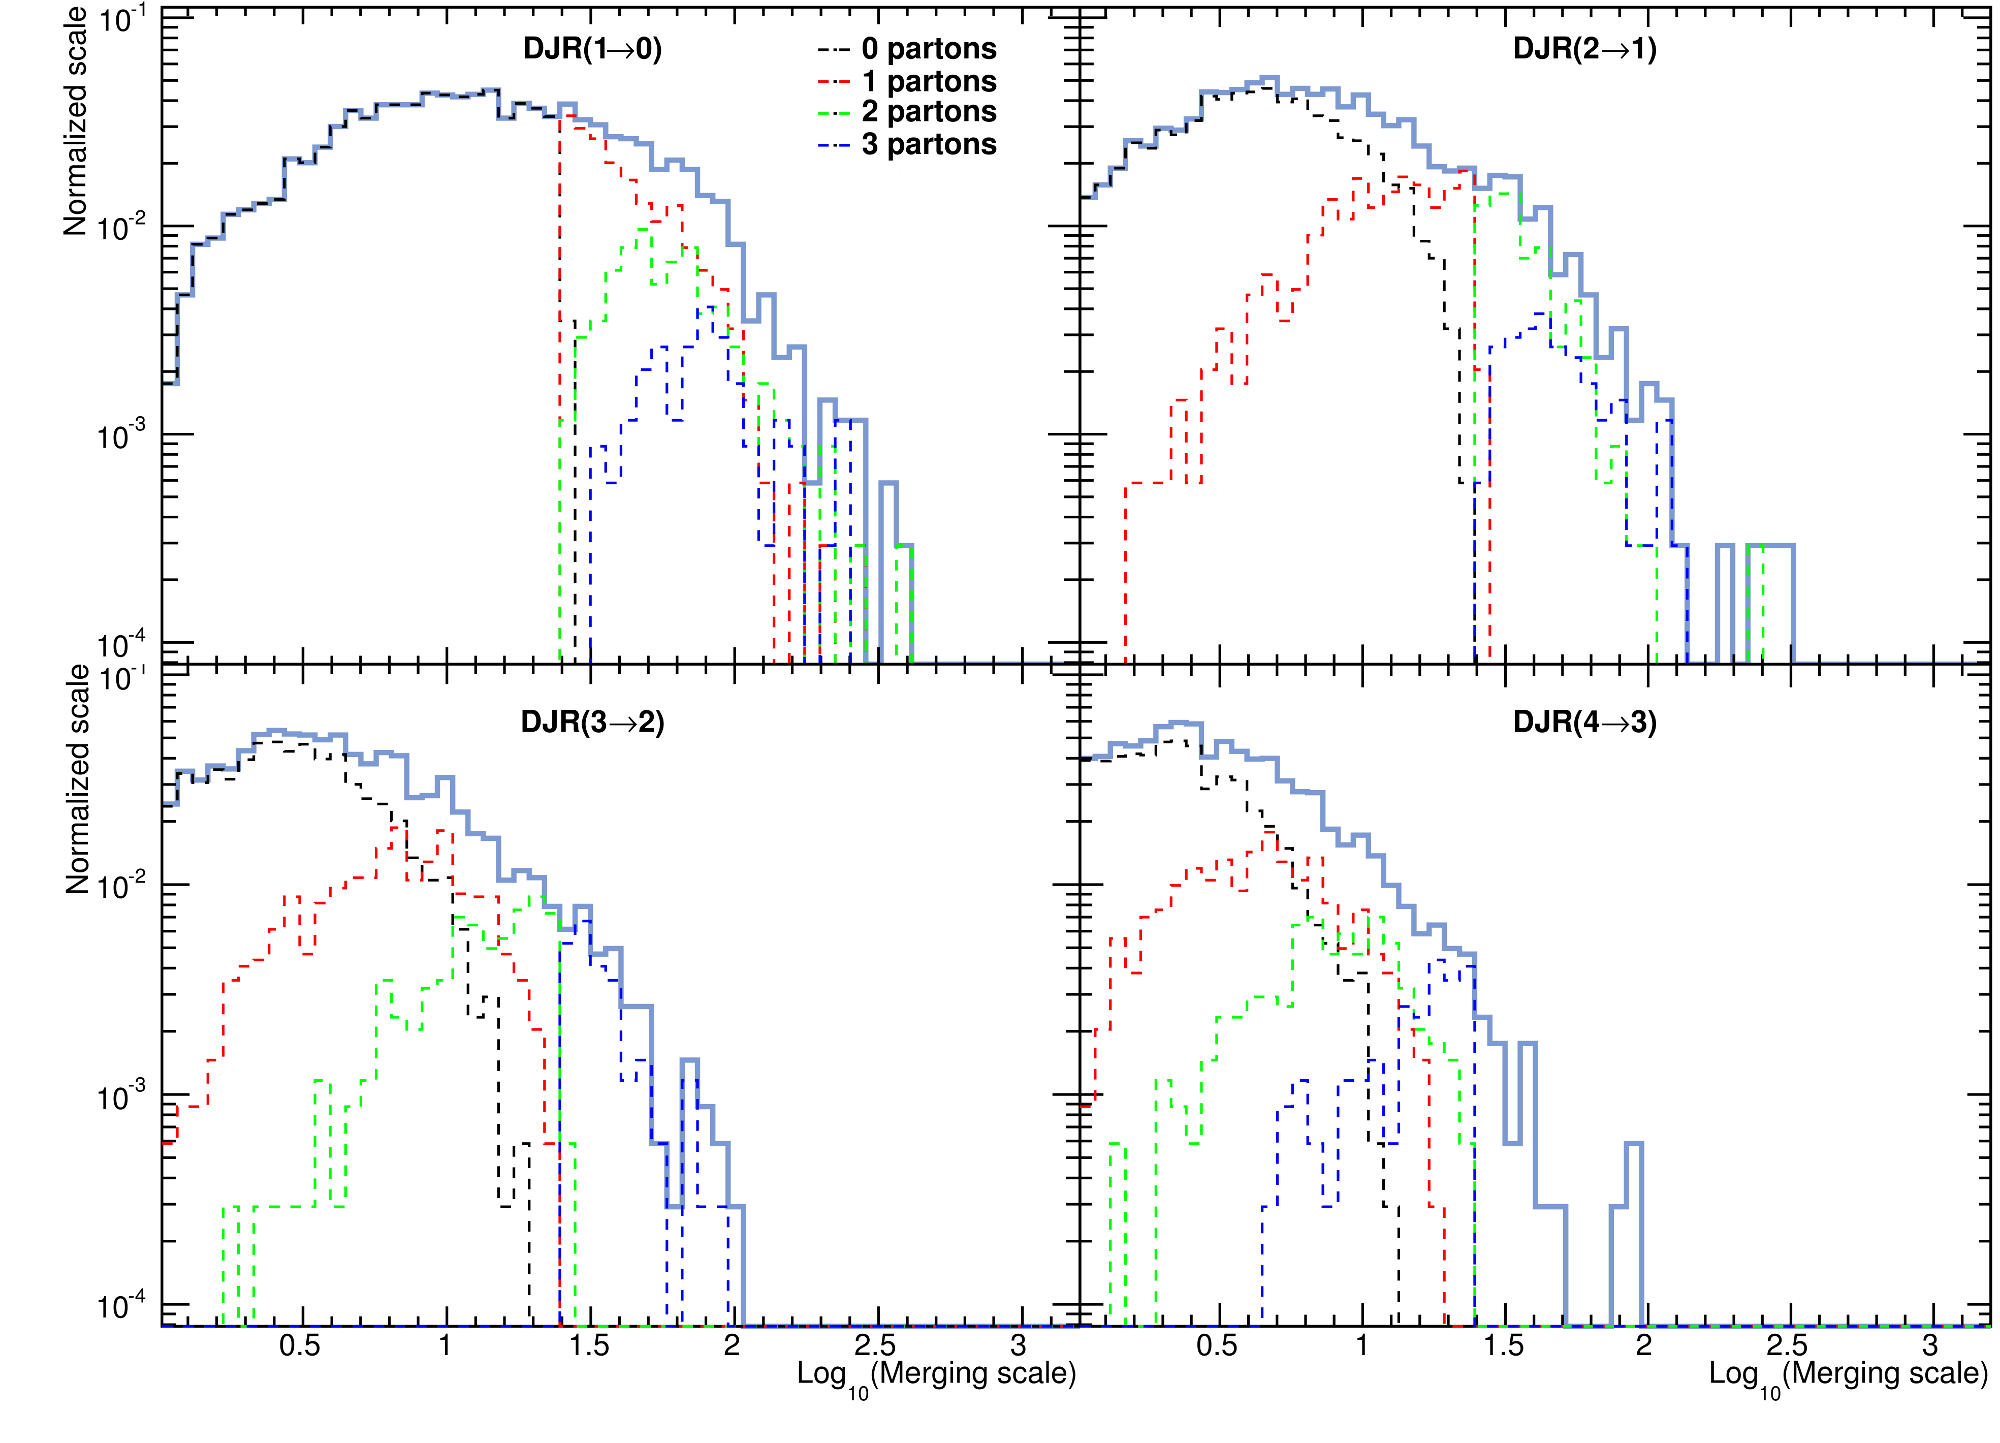
\includegraphics[width=0.85\textwidth]{figs/DJR_q25_xq10_DYJets13TeV.png}
    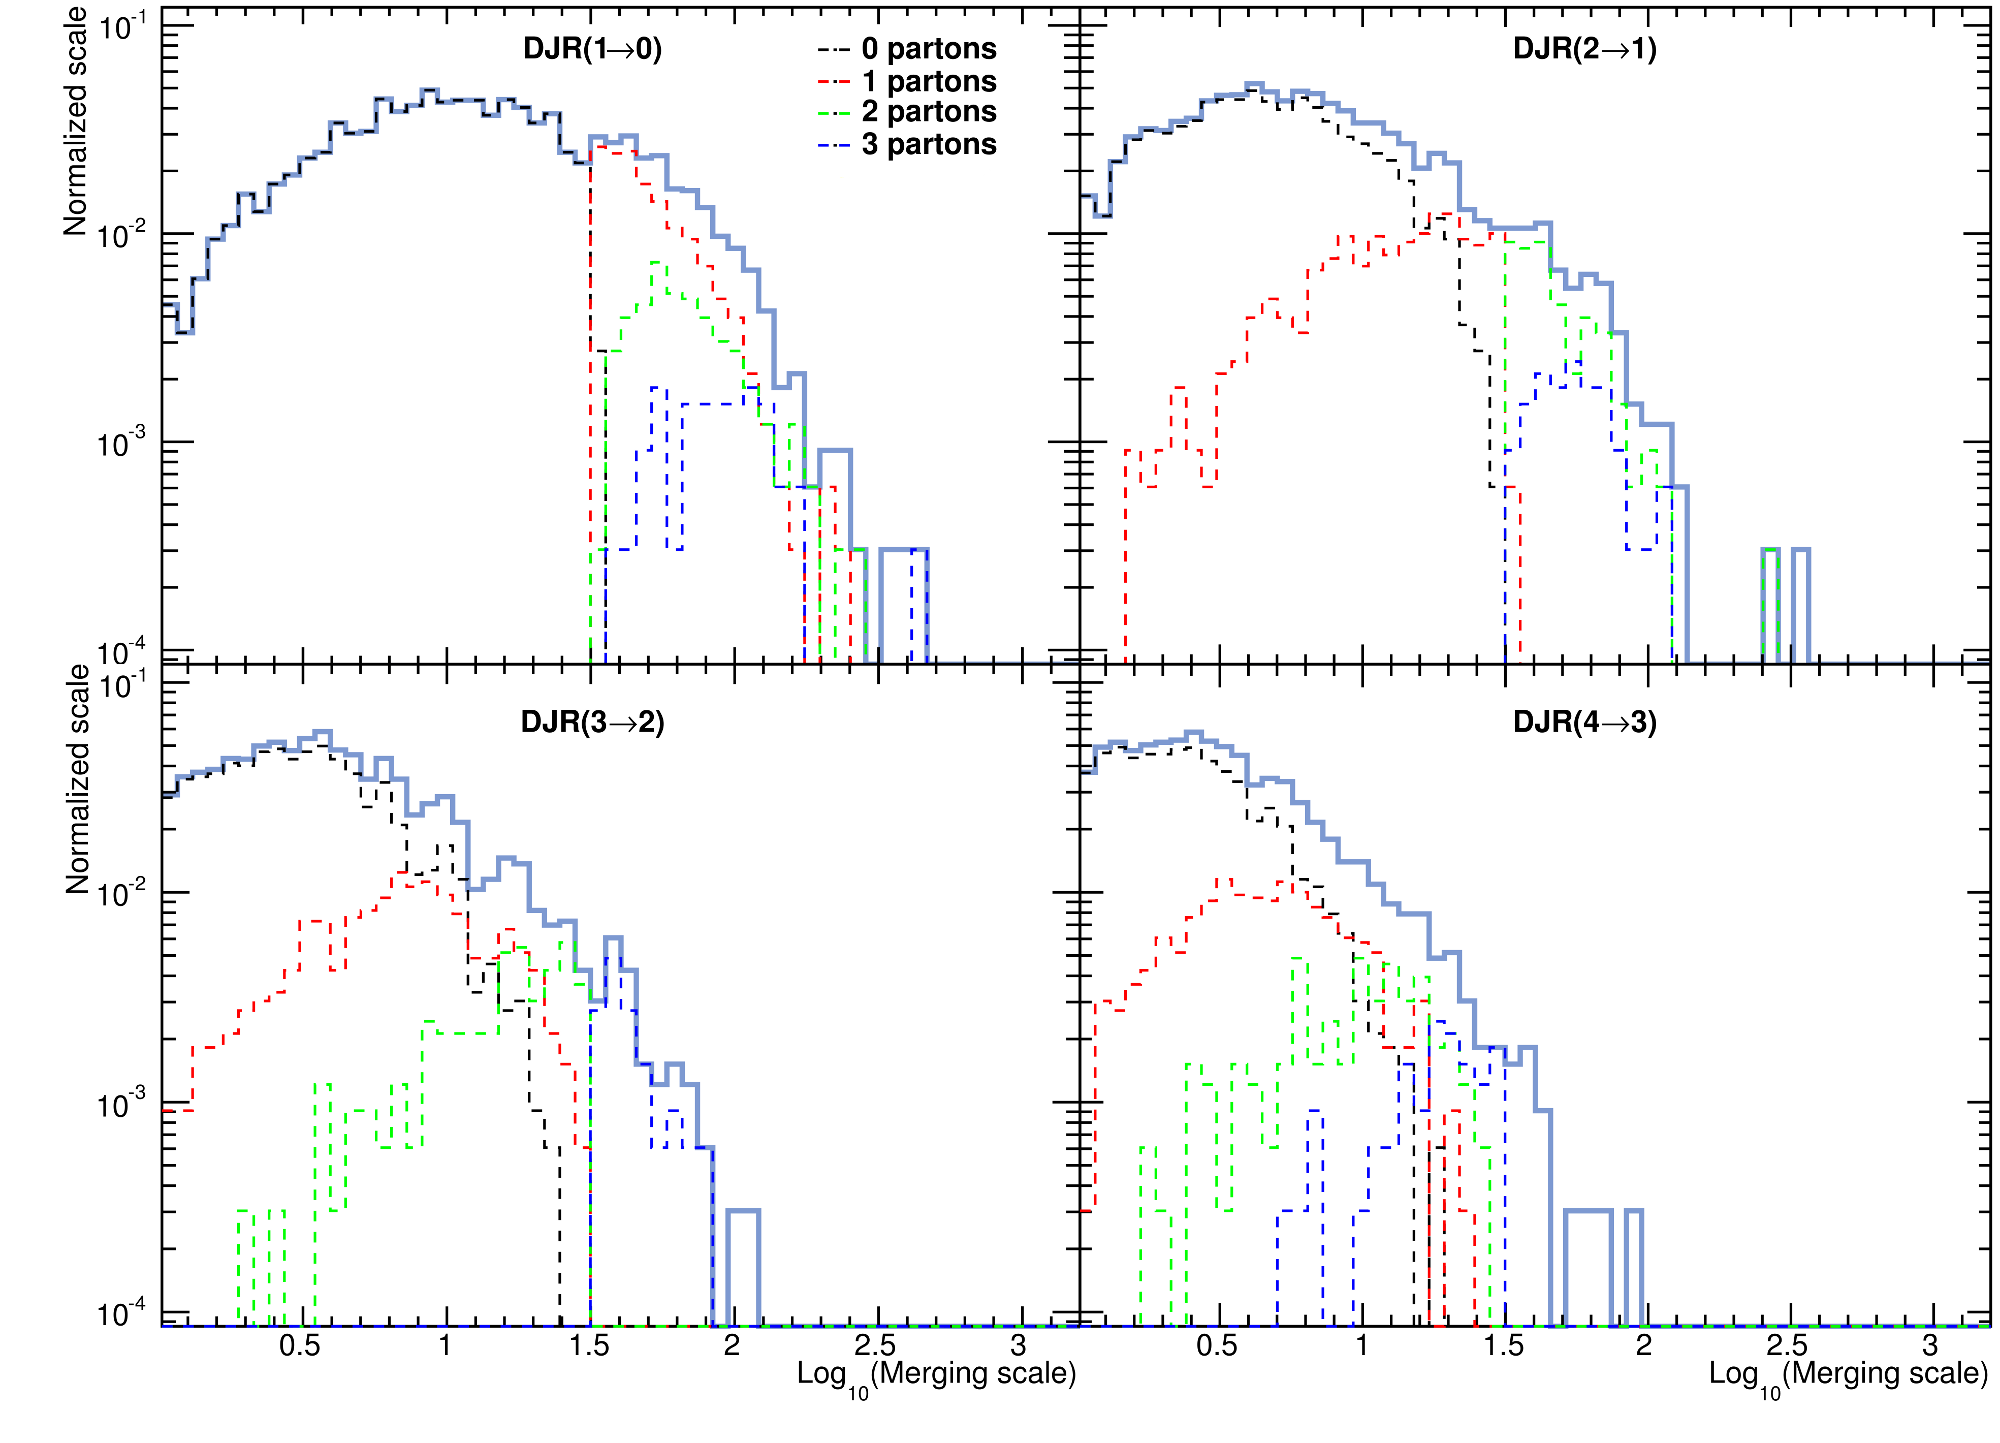
\includegraphics[width=0.85\textwidth]{figs/DJR_q32_xq10_DYJets13TeV.png}
    \caption{DJR diagrams for 13 TeV Drell-Yan production with $Q_{cut}=125$ GeV and $Q^{X}_{cut}=10$ GeV [optimal case] (top) and $Q_{cut}=32$ GeV and $Q^{X}_{cut}=10$ [non-optimal] (bottom). Bottom figure shows a discontinuity in the transition from 1 to 0 partons at the point where black-dashed and red-dashed curves meet.}
    \label{fig:DYMerging}
  \end{center}
\end{figure}

\section{Validation on data}
\label{sec:val}

MC simulations are theory based, in the sense that generated events reflect predictions of a given model. For example, the simulation of top quark decay depends on the theory predictions of the branching ratios of all its possible final states. Such branching ratios are utilized by generators as probabilities, to evaluate with random numbers if a top quark in a single event decay into a specific channel. 

A considerable number of SM processes have been measured by experiments very accurately. Such processes have also served to test theoretical predictions. Such well understood processes can be then used as reference to test the accuracy of MC simulations. All MC generators are tested against known experimental and theoretical results to prove their validity. For example, MadGraph versions used in CMS have been carefully validated internally by the collaboration before being used for central production.

\subsection{RIVET}
\label{sec:rivet}

There are different tools designed to validate MC generators. The Rivet project (Robust Independent Validation of Experiment and Theory)~\cite{Buckley:2010ar} is a toolkit for MC generators validation, providing a large set of experimental analyses. This tool has been extensively used by experiments and MC generators developers for MC development, tuning and validation. 

Rivet not only provides the analyses, it also provides the experimental data resulting from them. These data have been processed to unfold detector effects from them. This procedure tries to inverse detector simulation to obtain event information of particles before interacting with the detector. This constitutes a suitable method to compare data with MC simulations up to hadronization. ATLAS and CMS experiments contribute constantly by providing unfolded results to Rivet toolkit database.

Figures~\ref{fig:WVal} and~\ref{fig:ZVal} display examples of MC validation using Rivet tool. For the first figure, a comparison between several MC simulations have been compared to ATLAS experiment data in the measurement of \W~boson $p_{T}$. In figure~\ref{fig:ZVal}, the same MC generators have been compared to \Z~boson $p_{T}$ measurements performed by ATLAS and CMS. In the three validations, MadGraph interfaced with Pythia 6 describe better the real data than the other generators used. 

\begin{figure}[!Hhtbp]
  \begin{center}
    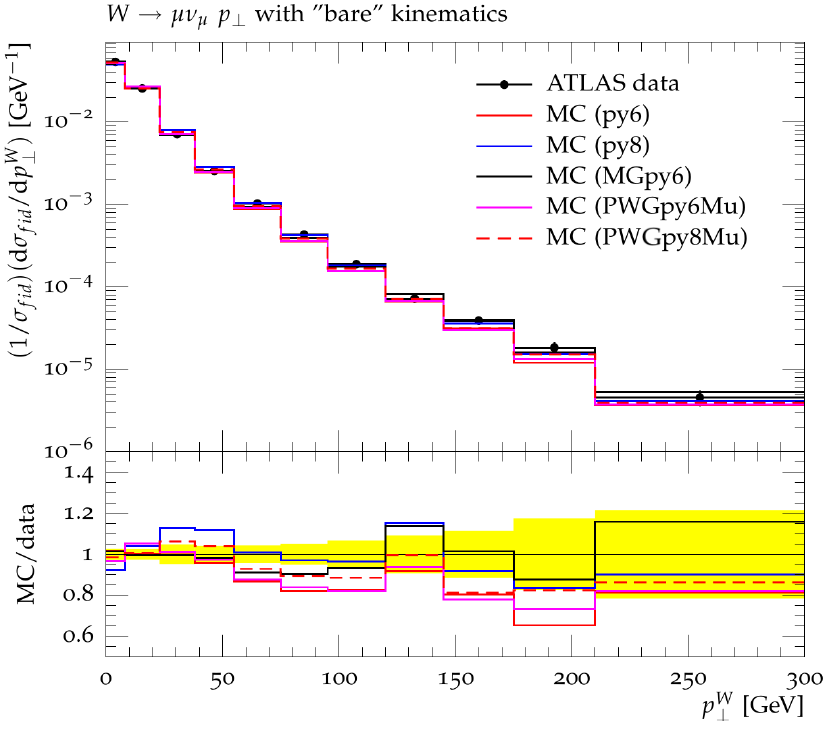
\includegraphics[width=0.55\textwidth]{figs/Wpt_rivet.png}
    \caption{\W~boson $p_{T}$ measured by ATLAS experiment in muon final states compared to different MC simulations. py6 stands for Pythia 6, py8 for Pythia 8, MGpy6 for MadGraph interfaced with Pythia 6 and PWG for Powheg. MadGraph with Pythia 6 gives the best description of experimental data for the shown observable.}
    \label{fig:WVal}
  \end{center}
\end{figure}

\begin{figure}[!Hhtbp]
  \begin{center}
    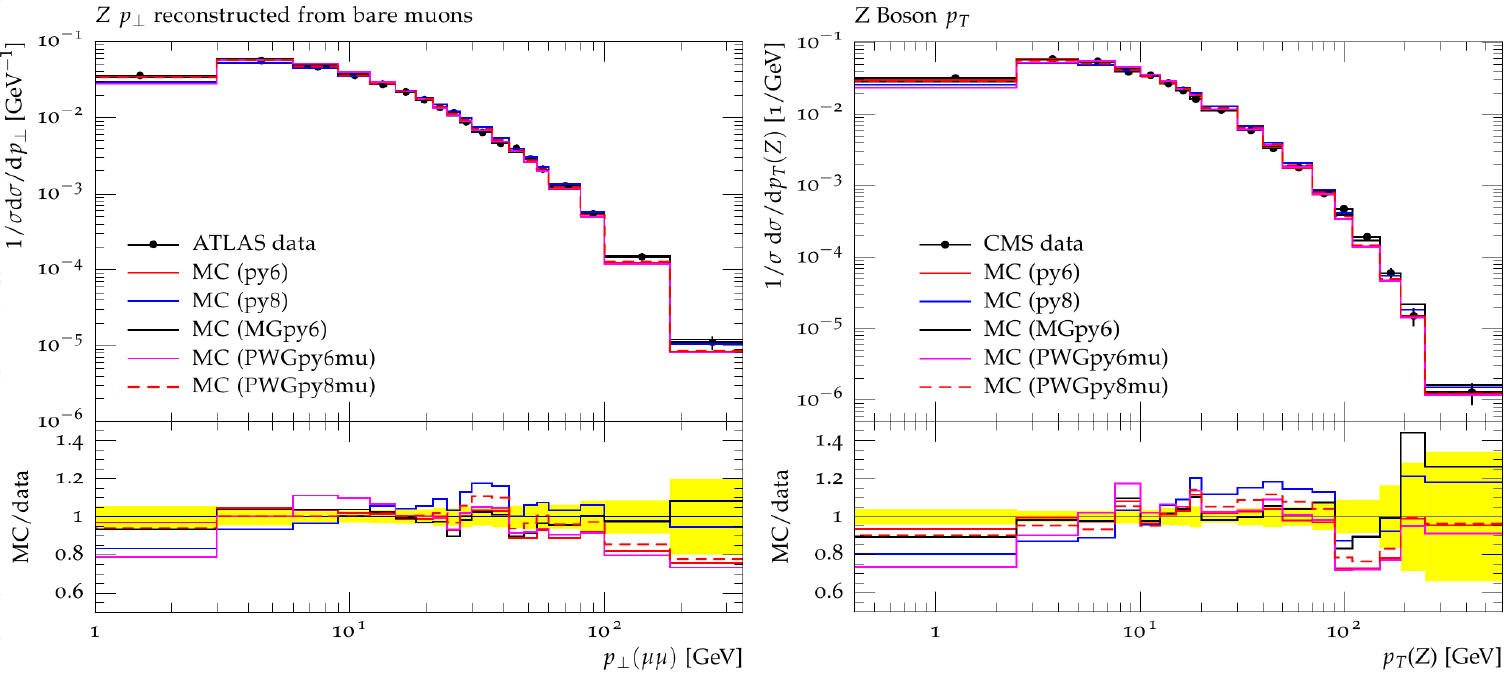
\includegraphics[width=1.0\textwidth]{figs/Zpt_rivet.png}
    \caption{\Z~boson $p_{T}$ measured by ATLAS [left] and CMS [right] experiments in di-muon channel. py6 stands for Pythia 6, py8 for Pythia 8, MGpy6 for MadGraph interfaced with Pythia 6 and PWG for Powheg. MadGraph with Pythia 6 gives the best description of experimental data in both cases.}
    \label{fig:ZVal}
  \end{center}
\end{figure}

In general, present MC generators describe correctly SM physics. However, there are known observables that are not correctly described by MC simulations. The most important issue has been seen when measuring the $p_{T}$ of the top quark in top-pair production. Figure~\ref{fig:TopPTReweighting} shows the ratio between data and MC, produced with MadGraph and Pythia 6, for the differential cross section of top pair production~\cite{Goerner:1754332}. This figure has been produced from the combination of different CMS analyses~\cite{Chatrchyan:2012saa,Chatrchyan:2013boa,Khachatryan:2015oqa}. A clear trend can be seen, showing that top $p_{T}$ in MC tend to be higher than in data. Due to this issue, MadGraph with Pythia 6 simulations of top pair production should be corrected. These corrections are considerable for high $p_{T}$ tops. They have been studied for tops with a $p_{T}$ smaller than 400 GeV/c.

\begin{figure}[!Hhtbp]
  \begin{center}
    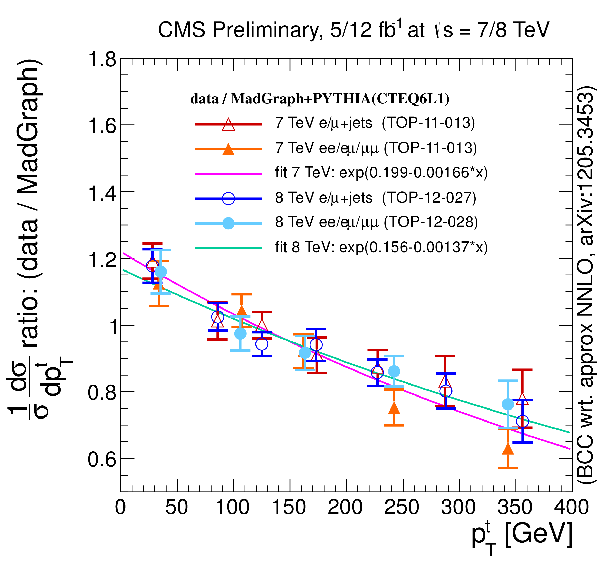
\includegraphics[width=0.6\textwidth]{figs/topPtDataOverMadgraphPythia.png}
    \caption{Data to MC ratio of normalized differential top pair production cross section as s function of top $p_{T}$. The \pt~of the top quark measured in MC tends to be higher than in data for a \pt~greater than 100 GeV/c~\cite{Goerner:1754332}.}
    \label{fig:TopPTReweighting}
  \end{center}
\end{figure}
%\begin{TOINCLUDE}Plot of W+jets and Z+jets comparison between data and MC for a set of different generators. Plot on top pt to briefly introduce tpo pt reweighting\end{TOINCLUDE}

In conclusion, though MC simulations are useful to understand particle physics processes and to test theoretical predictions, they are not always fully valid. For example, high $p_{T}$ spectra of particles or high jet multiplicity are not always well reproduced. For this reason it is very important for analyses looking for new physics that have to deal normally with non-explored or poorly explored physics, to develop strategies to estimate backgrounds from data. MC simulations are however useful to compare theoretical predictions with experimental measurements, in particular in this work they were used to model the signal characteristics in a search for a top-partner, described in chapter~\ref{chap:search}. 
